% Options for packages loaded elsewhere
\PassOptionsToPackage{unicode}{hyperref}
\PassOptionsToPackage{hyphens}{url}
%
\documentclass[
]{article}
\usepackage{amsmath,amssymb}
\usepackage{iftex}
\ifPDFTeX
  \usepackage[T1]{fontenc}
  \usepackage[utf8]{inputenc}
  \usepackage{textcomp} % provide euro and other symbols
\else % if luatex or xetex
  \usepackage{unicode-math} % this also loads fontspec
  \defaultfontfeatures{Scale=MatchLowercase}
  \defaultfontfeatures[\rmfamily]{Ligatures=TeX,Scale=1}
\fi
\usepackage{lmodern}
\ifPDFTeX\else
  % xetex/luatex font selection
\fi
% Use upquote if available, for straight quotes in verbatim environments
\IfFileExists{upquote.sty}{\usepackage{upquote}}{}
\IfFileExists{microtype.sty}{% use microtype if available
  \usepackage[]{microtype}
  \UseMicrotypeSet[protrusion]{basicmath} % disable protrusion for tt fonts
}{}
\makeatletter
\@ifundefined{KOMAClassName}{% if non-KOMA class
  \IfFileExists{parskip.sty}{%
    \usepackage{parskip}
  }{% else
    \setlength{\parindent}{0pt}
    \setlength{\parskip}{6pt plus 2pt minus 1pt}}
}{% if KOMA class
  \KOMAoptions{parskip=half}}
\makeatother
\usepackage{xcolor}
\usepackage[margin=1in]{geometry}
\usepackage{graphicx}
\makeatletter
\def\maxwidth{\ifdim\Gin@nat@width>\linewidth\linewidth\else\Gin@nat@width\fi}
\def\maxheight{\ifdim\Gin@nat@height>\textheight\textheight\else\Gin@nat@height\fi}
\makeatother
% Scale images if necessary, so that they will not overflow the page
% margins by default, and it is still possible to overwrite the defaults
% using explicit options in \includegraphics[width, height, ...]{}
\setkeys{Gin}{width=\maxwidth,height=\maxheight,keepaspectratio}
% Set default figure placement to htbp
\makeatletter
\def\fps@figure{htbp}
\makeatother
\setlength{\emergencystretch}{3em} % prevent overfull lines
\providecommand{\tightlist}{%
  \setlength{\itemsep}{0pt}\setlength{\parskip}{0pt}}
\setcounter{secnumdepth}{-\maxdimen} % remove section numbering
\ifLuaTeX
  \usepackage{selnolig}  % disable illegal ligatures
\fi
\IfFileExists{bookmark.sty}{\usepackage{bookmark}}{\usepackage{hyperref}}
\IfFileExists{xurl.sty}{\usepackage{xurl}}{} % add URL line breaks if available
\urlstyle{same}
\hypersetup{
  pdftitle={Simple, intuitive tool for population management decision-making},
  pdfauthor={Post provided by Izzy McCabe},
  hidelinks,
  pdfcreator={LaTeX via pandoc}}

\title{Simple, intuitive tool for population management decision-making}
\author{Post provided by Izzy McCabe}
\date{}

\begin{document}
\maketitle

Along with my colleagues Diego Rincon and Dave Crowder, we have just
published ``Sequential testing of complementary hypotheses about
population density'' in MEE. The idea started as an offshoot of our
research into improving site-specific predictions of Codling moth, a
prolific tree fruit pest. Conventional planning for pest management
typically involves a phenology model, which relates heat accumulation to
pest emergence after the winter, in combination with on-site sampling to
inform decisions about controlling pest populations. A drawback of
existing methods is that phenology and sampling remain unlinked; growers
use their intuition and experiences to connect the dots. The intuition
of experienced growers is not to be underestimated, and they are skilled
at knowing how pest counts by certain periods in the season are related
to seasons where management interventions are needed. We wanted growers
to be able to set their own maximum tolerable thresholds, and for us to
use our site-specific profiles in conjunction with early-season data to
predict the probability of exceeding those thresholds.

{[}Figure 1{]}

After surveying the state-of-the-art in sequential analysis, we found
limitations in existing methods. The most popular sequential data
analysis procedure is the Sequential Probability Ratio Test (SPRT),
introduced in 1945 by Abraham Wald, but it requires fixed sample sizes
and the specification of two non-complementary models (i.e.~tests if
average captures per sample are 8 vs 10, rather than them being greater
than or less than 9). Furthermore, the original methodology only
accounts for one-at-a-time sequential sampling and requires complicated
modifications to support group sequential designs that are inherent to
pest sampling networks. We believed that the problem of iteratively
updating our knowledge and predictions based on new data aligns with the
philosophy of Bayesian statistics, and sure enough we found methods
utilizing Bayes' Rule to the domain of sequential hypothesis testing in
Morgan \& Cressie's Variable Probability Ratio Test (VPRT). Their
method, while providing compelling optimality properties, still requires
non-complementary hypothesis ratios and comes with the computational
difficulties of Bayesian methods. Our new method, the Sequential Test of
Bayesian Posterior Probabilities (STBP) can be seen as building on the
VPRT and aims to provide an ergonomic and intuitive procedure that
explicitly supports variable sample sizes over time, explicit
threshold-style hypotheses, and even dynamic trajectories as hypotheses.

It works by making a crucial simplification of typical Bayesian methods:
instead of the specification of proper prior probability distributions,
it assigns a single probability to the parameter of inference being
greater (or less) than the threshold and the complementary probability
for it being less (or greater) than that threshold. This is in
comparison to the typical procedure of giving each possible value of the
parameter its own probability density. This reduces the resulting
posterior probability from an entire distribution to a single number,
which we can then plug back into the equation as the prior probability
for the next iteration. It also eliminates the difficult computational
exercise of integrating over constantly changing joint probability
density functions which forms the major limitation for typical Bayesian
methods. Integrals only need be calculated over your desired likelihood
function, for which all commonly used distributions already have
closed-form solutions in the form of their cumulative density functions!
While our method had a greater rate of false positives compared to the
SPRT in one-at-a-time sequential designs, it outperformed it when
sequential sampling bouts are made of multiple samples. In general, the
STBP requires less sampling and errors scaled more favorably with
increasing sample sizes at each sampling time than the SPRT. We also
tested our method as a procedure for invasive species monitoring, where
it demonstrated higher power for equal sample sizes than conventional
approaches, with further reductions in required sampling when prior
belief in the absence of the invasive species is already high. We also
found that our simplified model quickly converges on the results
produced by more complex Bayesian techniques requiring proper conjugate
priors just by increasing sample size.

{[}Figure 2{]}

Because our method allows for both variable sample sizes and sequential
comparisons for changing-but-related hypotheses, it also has potential
applications in continuous monitoring for signal processing, fraud
detection, forensics, and clinical tests (like that of changes in
glucose levels, heart rate, or mortality). For example, by continuously
comparing the expected patient mortality rates for certain surgical
procedures to that of individual surgeons, we found that
\href{https://en.wikipedia.org/wiki/Harold_Shipman}{Harold Shipman's
serial killings} could have been detected with great confidence as early
as in early 80s for female victims and early 90s for male victims.
Unfortunately, the infamous ``Dr.~Death'' was convicted as late as in
January 2000 when he had killed nearly 300 people.

{[}Figure 3{]}

Our method represents innovation in a section of the ecological and
agricultural literature which has remained largely stagnant for many
decades. The SPRT, introduced in 1945, is still the most widely used
method for sequential analysis, and the fixed-sample size method used in
invasive species monitoring has been used unchanged since its
introduction in 1993. We plan on working to integrate the STBP into
integrated pest management strategies in the Pacific Northwest, and hope
to see others find places in their corners of science and industry where
it can improve their processes and research. To facilitate this, we are
working on an R package that will be easy to use and extensible. The
source code can be found in this
\href{https://github.com/rincondf/STBP}{GitHub repository}, and we will
be working to release an R package to the CRAN repository in the coming
weeks.

\begin{figure}
\centering
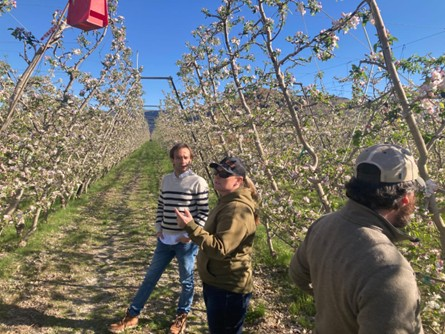
\includegraphics{Figures/Fig1Post.jpg}
\caption{\emph{Typical apple orchard in the state of Washington (USA),
where pest management decisions are made based on growers' intuition
combined with phenology models and moths captured in traps. Photo taken
by Tobin Northfield.}}
\end{figure}

\begin{figure}
\centering
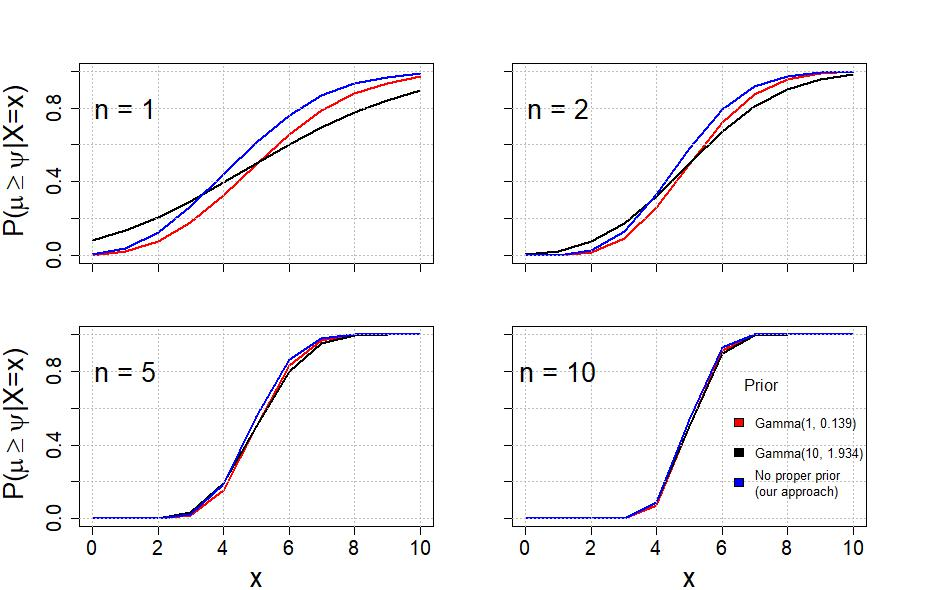
\includegraphics{Figures/Fig2Post.jpeg}
\caption{\emph{Comparison between posterior probabilities for a Poisson
random variable obtained from two configurations of Gamma conjugate
priors (black and red curves) and our approach, which omits an explicit
density function for \(\mu\) and includes a single probability of
\(P(\mu \ge \psi)\) (blue curves). As sample size increases, all models
converge to a similar set of posterior probabilities and the requirement
of specifying conjugate priors relaxes. R code for this analysis is
\href{https://github.com/rincondf/STBP/blob/403d7b559543d0f1f33097755c0dc253affbe5ea/Comparison_priors.R}{here}.}}
\end{figure}

\begin{figure}
\centering
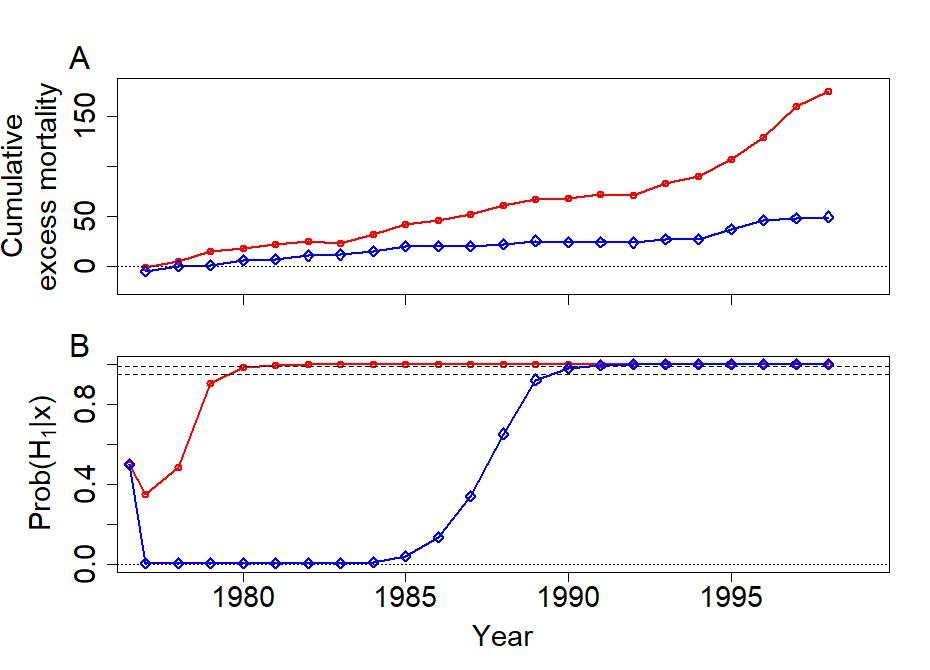
\includegraphics{Figures/Fig3Post.jpeg}
\caption{\emph{(A) Cumulative excess mortality, from the difference
between death certificates signed by Harold Shipman and expected
mortality in Wales, between 1977 and 1998 for male (blue) and female
(red) patients aged 65 or older. (B) Sequential Test of Bayesian
Posterior Probabilities for the hypothesis H1 that death certificates
signed by Shipman exceed by 33\% or more the expected mortality rates in
Wales for males or females aged 65 or older. Horizontal dashed lines
denote probabilities of 0.95 and 0.99. So, by 1980 for females and 1990
for males, there was \textgreater{} 95\% chance ``Dr.~Death'' had signed
at least 33\% more death certificates for patients aged 65 or older than
the average of practitioners in Wales. Data was extracted from
\href{https://www.researchgate.net/publication/320035425_Harold_Shipmans_clinical_practice_1974-1998_A_clinical_audit_commissioned_by_the_Chief_Medical_Officer}{Baker
\& Donaldson (2001)} and the R code for this analysis is
\href{https://github.com/rincondf/STBP/blob/403d7b559543d0f1f33097755c0dc253affbe5ea/ShipmanAnalysis.R}{here}.}}
\end{figure}

\end{document}
